\section{Confirmation Results}
\label{sec:results}

All 4,040 confirmation responses received three valid event codes, yielding
12,120 coder outputs and 32,320 majority-coded response--event observations.
The six disclosed larger-budget codes are included; the original failures are
retained. On this complete panel, pairwise positive coder agreement is
99.05--99.29\% for answer revelation, 91.38--92.52\% for reasoning elicitation,
and 96.29--98.15\% for affect acknowledgement. These are measurement diagnostics
over all arms, distinct from the repeated-generation agreement below.

\subsection{Different Defaults, Uneven Repetition (RQ1)}

On the 32 canonical source problems, the deployments differ substantially in
their action frequencies (Table~\ref{tab:default-rates}). GLM reveals an answer
in 22.3\% of responses and elicits reasoning in 96.5\%; DeepSeek and Doubao
reveal answers in every response, with elicitation below 5\%. M3 combines
both actions in 81/256 responses (31.6\%). These pooled profiles need not distinguish every
model pair: DeepSeek and Doubao have the same observed answer-revelation rate.

\begin{table}[t]
\centering\small
\begin{tabular}{lrrr}
\toprule
Deployment & Reveal & Elicit & Acknowledge \\
\midrule
MiniMax-M2.7 & 99.6 & 8.2 & 27.0 \\
MiniMax-M3 & 83.2 & 48.4 & 69.9 \\
DeepSeek-V4-Pro & 100.0 & 2.0 & 59.0 \\
Doubao-Seed-2.0-Lite & 100.0 & 4.3 & 60.9 \\
GLM-5.3 & 22.3 & 96.5 & 51.2 \\
\bottomrule
\end{tabular}
\caption{Canonical event rates (\%): 256 answers per deployment, eight per
source, on 32 sources. Events can co-occur. Abbreviated deployment names in the
text refer to these configurations, not all releases in their model families.}
\label{tab:default-rates}
\end{table}

Recurring distributions do not imply identical actions on repeated requests.
M3's elicitation agreement is only 57.8\% across 128 matched input pairs
(95\% source-bootstrap interval 50.0--66.4\%). Conversely, DeepSeek and Doubao
have 96.1\% and 91.4\% elicitation agreement but zero positive agreement:
their few positive occurrences do not recur in both requests. Perfect answer
agreement for these two deployments reflects an observed ceiling. We therefore
interpret recurrence through prevalence, agreement on presence and absence,
and prospective prediction together (Appendix~\ref{app:confirmation-details}).
Appendix~\ref{app:materials-examples} provides a same-input response set,
including a coding disagreement, to illustrate the event distinctions.

\subsection{Defaults Transfer; Conditional Gains Are Selective (RQ2)}

All three model-default predictors improve over the situation-only baseline
on new sources (Figure~\ref{fig:primary-gains}). The absolute Brier reductions
are 0.09127 for revelation, 0.12970 for elicitation, and 0.01982 for
acknowledgement; all pass the six-test Holm correction. Absolute losses fall
from 0.15359 to 0.06232, 0.21873 to 0.08903, and 0.18242 to 0.16260,
respectively. Thus the identity-specific information learned before confirmation
predicts actions beyond the supplied subject and student-state context.

\begin{figure}[t]
\centering
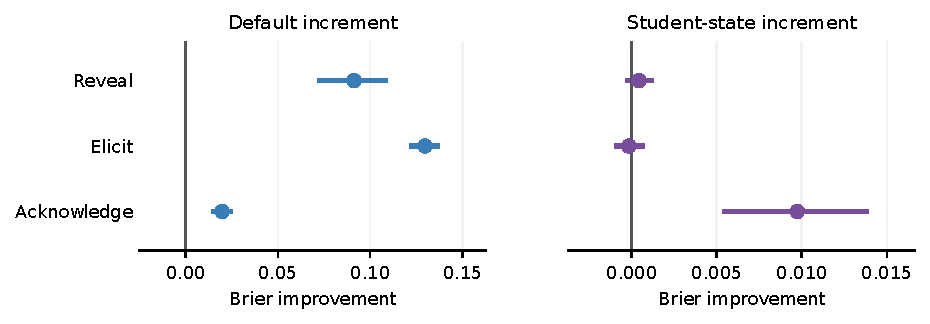
\includegraphics[width=\linewidth]{figures/confirmation_prediction_gains_publication.pdf}
\caption{All six primary predictive comparisons on 32 new source problems.
Positive values denote lower Brier loss. Lines show 95\% source-bootstrap
intervals conditional on the fitted training profiles; they are not simultaneous
intervals. The panels use different horizontal scales. Exact gains, intervals,
and six-test Holm-adjusted one-sided $p$-values appear in
Table~\ref{tab:primary-tests}.}
\label{fig:primary-gains}
\end{figure}

Adding model-specific student-state responses to model-by-subject profiles
gives a different result. Acknowledgement improves by 0.00973
(95\% interval [0.00536, 0.01395], adjusted $p=0.000192$), reducing Brier loss
from 0.16046 to 0.15072. Revelation gains only 0.00043
([-0.00037, 0.00130], $p=0.326$); elicitation changes by -0.00016
([-0.00101, 0.00073], $p=0.641$). These unresolved increments concern
the specified cues and predictor class, not every possible form of adaptation.

The acknowledgement profiles clarify the positive conditional result. For
correct unfinished work, Doubao acknowledges difficulty in 0/64 calm responses
and 60/64 frustrated responses; DeepSeek changes from 22/64 to 34/64.
For erroneous work, their corresponding changes are 32/64 to 64/64 and
46/64 to 49/64. These are responses to scripted text cues, not measurements
of empathy or learner understanding. The descriptive curves appear in
Appendix~\ref{app:confirmation-details}; the locked prediction comparison
provides the test that such model-specific patterns recur on new sources.

The training-only length/formatting competitor yields losses of 0.13861,
0.17826, and 0.17864 for the three events, exceeding the model-default losses
in each case. This descriptive comparison shows that two simple style summaries
do not reproduce the predictive result. It neither excludes richer stylistic
explanations nor identifies a causal effect of model identity.

\subsection{Instructions Converge on Demanded Actions (RQ3)}

The matched prompt comparison uses 16 sources and 128 answers per deployment
per arm. ASK requires eliciting a next step without stating the final answer.
All five deployments elicit reasoning in all 128 ASK responses. Revelation
falls to zero for DeepSeek, Doubao, and GLM, but remains in 9/128 M2.7 and
4/128 M3 responses. EXPLAIN instead requires a solution and final answer,
while explicitly permitting follow-up reasoning or questions. Every deployment
reveals the answer in every EXPLAIN response.

Convergence on the requested action does not eliminate all observed differences.
Under EXPLAIN, elicitation occurs in 62.5\% of GLM and 45.3\% of M3 responses,
compared with 1.6--5.5\% for the other three deployments. Since all these
responses reveal the answer, those rates also describe joint revelation and
elicitation. This permitted behavior is not an instruction violation, and the
event codes do not establish its temporal order. A single answer-versus-question
axis would hide it. Matched rates and paired prompt changes are reported in
Appendix~\ref{app:confirmation-details}.

Neutral role paraphrases place a further limit on stable-type interpretations.
For GLM, neutral B raises both revelation and acknowledgement by 15.6 percentage
points relative to the matched canonical arm. These are observed shifts, not
additional primary tests. No neutral comparison establishes population
equivalence within $\pm 0.10$ under the disclosed bounded-source check: with
16 sources its simultaneous half-width is 0.9414. This lack of precision
cannot be used as evidence for either universal stability or universal wording
sensitivity.

\subsection{Dependence on Measurement and Model Composition}

Eight coding panels preserve the broad separation between default and
student-state increments. Default-gain estimates range from 0.08571--0.09562
for revelation, 0.12442--0.13111 for elicitation, and 0.01699--0.02017 for
acknowledgement. Conditional acknowledgement gains range from
0.00697--0.01052; conditional revelation and elicitation remain near zero.
These reuse the same outputs and are sensitivity estimates, not independent
replications.

Effect strength depends materially on which deployments are included.
Deleting GLM reduces default gains to 0.00394 for revelation and 0.03080 for
elicitation. Deleting M2.7 reduces the acknowledgement default gain to 0.00175,
with an interval crossing zero [-0.00174, 0.00547]. The full-panel findings
therefore do not imply equally strong differences among every subset of models.
Across 200 training-source resamples, the descriptive 2.5--97.5 percentile
range for conditional acknowledgement gain is [0.00542, 0.01039]; revelation
spans zero and elicitation remains slightly negative. These distributions
condition on fixed confirmation labels and the original regularization ratio.

The six confirmation budget exceptions do not determine the primary findings.
For either binary value of each affected canonical GLM code, all six primary
estimates and adjusted $p$-values are exactly unchanged: the other two coders
agree on the three primary events. This fixed-prediction enumeration addresses
those missing codes only. It does not validate coder behavior across the
Gateway interruption. Complete secondary results and sensitivity ranges are
retained in Appendix~\ref{app:confirmation-details}.

\paragraph{Mathematics and content screening.}
The mathematics subset (eight sources, 320 responses) retains default gains
of 0.11624, 0.13892, and 0.01992; student-state increments are 0.00062,
0.00030, and 0.01380 for revelation, elicitation, and acknowledgement.
All 2,584 content reviews are valid after the disclosed structural repairs.
Excluding five-model slots flagged by either reviewer retains 1,065 responses
on all 32 sources. Default gains are 0.09535, 0.13179, and 0.02068;
conditional acknowledgement gains 0.00989 [0.00510, 0.01472], while the
other two conditional intervals span zero. The unanimous-error screen retains
1,255 responses and the same qualitative pattern. No uncertainty verdicts
occur, so the error-or-uncertainty screen is identical to the either-error
screen (Appendix~\ref{app:content-results}).

These are descriptive selected-subset estimates, with no new tests. Both
reviewers match all twelve diagnostic controls, yet agree on an error in only
5 of the 49 natural responses flagged by either (positive agreement 18.5\%).
Screening thus tests sensitivity to these judgments; it neither guarantees
correct remaining answers nor causally separates behavior from ability.
